\documentclass[12pt,a4paper]{article}

\usepackage[utf8]{inputenc}
\usepackage[russian]{babel}
\usepackage[OT1]{fontenc}
\usepackage{amsmath}
\usepackage{amsfonts}
\usepackage{amssymb}
\usepackage{graphicx}
\usepackage{tikz}
\usepackage{pgfplots}
\usepackage[export]{adjustbox}
\usepackage{wrapfig}
\usepackage[left=2cm,right=2cm,top=2cm,bottom=2cm]{geometry}
\usepackage{setspace}
\usepackage{booktabs}
\usepackage{multirow}

\begin{document}

\title{
2.1.3.

Определение $C_p/C_v$ по скорости звука в газе.
\author{Семёнов Андрей Б02-016}
}
\date{21 апреляля 2021г.}

\maketitle

\newpage


\textbf{Цель работы:} 1) Измерение частоты колебаний и длины волны при резонансе звуковых колебаний в газе, заполняющем трубу; 
2) Определение показателя адиабаты с помощью уравнения состояния идеального газа.

\textbf{В работе используются:} звуковой генератор ГЗ, электронный осциллограф ЭО, микрофон, телефон, раздвижная труба, теплоизолированная труба, обогреваемая водой из термостата, баллон со сжатым углекислым газом, газгольдер.

\section{Теоретические сведения}
Из теории нам известна зависимость скорости звука от показателя адиабаты $\gamma$:
$$c = \sqrt{\gamma\frac{RT}{\mu}}.$$
Таким образом, задача нахождения $\gamma$ сходится к задаче нахождения скорости звука при заданной температуре.\\
В этом эксперименте предпологается использовать стоячие волны для нахождения $c$. Известно, что стоячие волны в коридоре длиной $L$ образуются при:
$$L = \frac{n}{2}\lambda,$$
где $\lambda$ -- длина волны звука, связанная со скоростью звука и частотой $f$, как:
$$\lambda = c/f.$$
То есть верно, что:
$$L = \frac{c}{2f}n.$$

При неизменной частоте f звукового генератора (а следовательно, и неизменной длине звуковой волны $\lambda$) можно изменять длину трубы $L$. Для этого применяется раздвижная труба. Длина раздвижной трубы постепенно увеличивается, и наблюдается ряд последовательных резонансов. Для $k$-ого резонанса имеем:
$$L_{n+k}=n\frac{\lambda}{2} + k\frac{\lambda}{2},$$
т. е. $\lambda/2$ равно угловому коэффициенту графика, изображающего зависимость длины трубы $L$ от номера резонанса $k$.
		
При постоянной длине трубы можно изменять частоту звуковых колебаний. В этом случае следует плавно изменять частоту $f$ звукового генератора, а следовательно, и длину звуковой волны $\lambda$.
Для $k$-ого резонанса получим:
$$L = (n+k)\frac{\lambda_{k+1}}{2}$$
$$f_{k+1} = \frac{c}{\lambda_{k+1}}=\frac{c}{2L}(n+k)=f_1 + \frac{c}{2L}k.$$
		
Скорость звука, деленная на $2L$, определяется, таким образом, по угловому коэффициенту графика зависимости частоты от номера резонанса.

В текущем эксперименте мы будем знать не абсолютный номер порядка $n$, а его приращение $k = n - n_0$, для которого верно, что:
$$\Delta L = L - L_0 = \frac{c}{2f}k + \Delta L_0,$$
где $L_0$ -- минимальный размер трубы, а $\Delta L$ -- отклонение от него, которое мы можем измерить.


\section{Экспериментальная установка}
В этой работе мы будем измерять зависимость $\Delta L(k)$ при постоянных значениях $f$, из чего получим $c$. Для этого мы используем установку на Рис. 1. Эта установка представляет из себя две вложенных друг в друга трубы с миллиметровой шкалой на подвижной части. На краях этой системы установлены приемник Т и передатчик М. Также к системе подведена трубка, через которую можно накачивать пространство внутри труб воздухом или углекислым газом.
\begin{center}
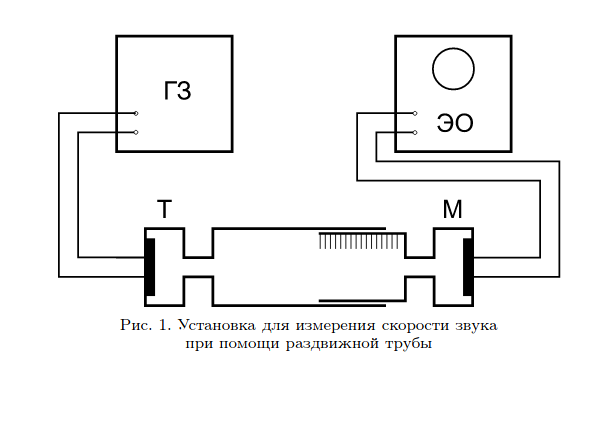
\includegraphics[width=0.95\textwidth]{equip.png}.
\end{center}


\section{Выполнение работы}


Сперва запишем параметры установки:
$L = 570\pm5 \; {мм}.$\\

Затем включим звуковой генератор с осциллографом и дадим им прогреться 5-7 минут.\\
Зададим амплитуду и частоту сигнала на генераторе так, чтобы на осциллографе можно было пронаблюдать сигнал. Он должен быть неискаженным синусоидальным. Если он будет искаженным, уменьшим амплитуду.\\

\textbf{Измерение скорости звука в воздухе.}\\
При изменении длины в $230 \text{мм}$, для того, чтобы при скорости в $340\text{м}/\text{с}$ было $\approx 4$ резонанса, нужна частота порядка:
$$f \approx \frac{4\cdot340\text{м}/\text{с}}{2 \cdot 0.23 \text{м}} \approx 3\text{кГц}.$$\\
Продуем трубу воздухом $\approx 5 \text{мин}$.\\
Для нескольких частот получим различные зависимости $\Delta L(k)$, плавно вытягивая и втягивая внутреннюю трубку относительно внешней и наблюдая за амплитудой показаний осциллографа. При достижении максимума амплитуды, наблюдается резонанс, и мы записываем новое значение $\Delta L$.

\begin{center}
\begin{tabular}{|c|c|c|c|c|c|c|c|c|c|c|c|}
\hline $N_\text{изм}$&$f, \text{кГц}$&$L(0),$ мм&$L(1),$ $\text{мм}$&$L(2),$ $\text{мм}$&$L(3),$ $\text{мм}$&$L(4),$ $\text{мм}$&$\lambda, \text{мм}$&$\Delta \lambda,$ $\text{мм}$&$c,$ $\text{м}/\text{с}$&$\Delta c,$ $\text{м}/\text{с}$&примечание\\ \hline
1&3.49&28&72&130&180&230&88.4&0.2&354&2&вверх\\ \hline
2&2.50&55&125&195&-&-&86.2&0.5&344&3&вниз\\ \hline
3&4.00&42&86&130&173&217&140.6&1.1&344&4&вверх\\ \hline
4&4.5&52&130&168&191&205&132.2&10.7&324&27&вниз\\ \hline
\end{tabular}
\end{center}


Приборная погрешность у этого эксперимента сопоставима с погрешностью мнк:
$$\varepsilon f \approx \frac{1}{200} = 0.5\%,$$
$$\varepsilon L \approx \frac{0.5}{100} = 0.5\%,$$
что добавит дополнительные $1\%$ погрешности к финальному результату.\\
\begin{figure}[h]
    \centering
    \begin{center}
    \end{center}
    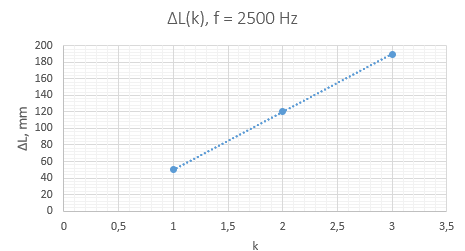
\includegraphics[width=10 cm]{plot1.PNG}
    \label{fig:plot1}
\end{figure} 
\begin{figure}[h]
    \centering
    \begin{center}
    \end{center}
    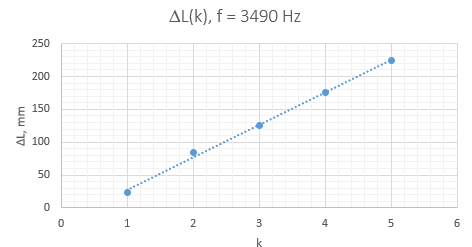
\includegraphics[width=10 cm]{plot2.PNG}
    \label{fig:plot2}
\end{figure} 
\begin{figure}[h]
    \centering
    \begin{center}
    \end{center}
    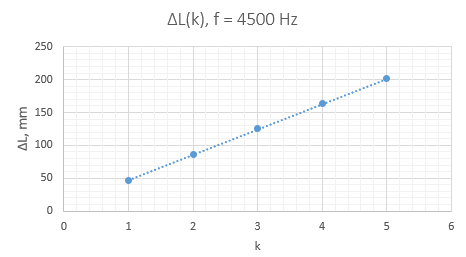
\includegraphics[width=10 cm]{plot3.PNG}
    \label{fig:plot3}
\end{figure} 
\begin{figure}[h]
    \centering
    \begin{center}
    \end{center}
    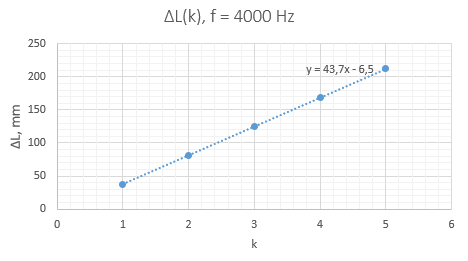
\includegraphics[width=10 cm]{plot4.PNG}
    \label{fig:plot4}
\end{figure} 
\newpage

Из МНК получается средняя скорость звука:
$$c = (350\pm3)\frac{\text{м}}{\text{с}}.$$

\textbf{Измерение скорости звука в углекислом газе.}\\
Измерение скорости звука в углекислом газе проводится аналогично скорости звука в воздухе, но со своими особенностями: установка не является герметичной, и поэтому в нее поступает воздух при движении трубы наружу. Поэтому метод нахождения получает новые особенности:

Просто открытия краника для того, чтобы закачать $CO_2$, недостаточно -- надо открыть краник и начать вводить-выводить внутреннюю трубу где-то 20 секунд, прокачивая $CO_2$ внутрь, и удаляя воздух.
 Измерения проводятся только при входе трубы внутрь. Поскольку измерения при полностью открытом кране невозможны из-за сильного шума на осциллографе, при выводе трубы, в установку закачивается воздух.\\
Во время измерений краник немного приоткрыт -- достаточно, чтобы был доступ к $CO_2$, но недостаточно, чтобы были помехи в работе осциллографа.

\begin{center}
\begin{tabular}{|c|c|c|c|c|c|c|c|c|c|c|c|c|}
\hline $N_\text{изм}$&$f, \text{кГц}$&$L(0),$ мм&$L(1),$ $\text{мм}$&$L(2),$ $\text{мм}$&$L(3),$ $\text{мм}$&$L(4),$ $\text{мм}$&$L(5),$ $\text{мм}$&$\lambda, \text{мм}$&$\Delta \lambda,$ $\text{мм}$&$c,$ $\text{м}/\text{с}$&$\Delta c,$ $\text{м}/\text{с}$&примечание\\\hline
1&3.25&8&48&89&132&172&212&82.0&0.4&266&2&\\ \hline
2&3.02&12&64&118&174&-&-&108.0&0.9&327&4&без п.2\\ \hline
3&2.74&35&90&149&207&-&-&115.0&0.8&315&3&без п.2\\ \hline
4&2.74&40&88&138&185&-&-&97.0&0.5&266&2&\\ \hline
5&2.23&32&92&153&212&-&-&120.2&0.4&268&2&\\ \hline
6&1.75&78&155&-&-&-&-&154.0&0.1&270&2&\\ \hline
7&1.50&8&105&188&-&-&-&180.0&4.7&271&9&\\ \hline
8&1.99&45&115&177&-&-&-&132.0&2.7&263&7&\\ \hline
9&2.50&55&105&160&213&-&-&105.8&1.0&264&3&\\ \hline
\end{tabular}
\end{center}
\begin{figure}[h]
    \centering
    \begin{center}
    \end{center}
    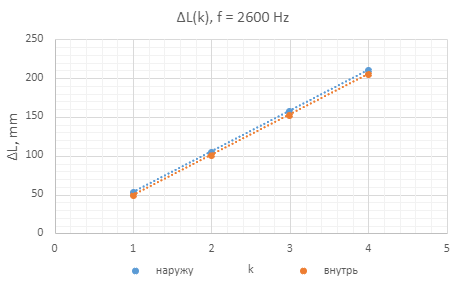
\includegraphics[width=10 cm]{coplot1.PNG}
    \label{fig:coplot1}
\end{figure}
\begin{figure}[h]
    \centering
    \begin{center}
    \end{center}
    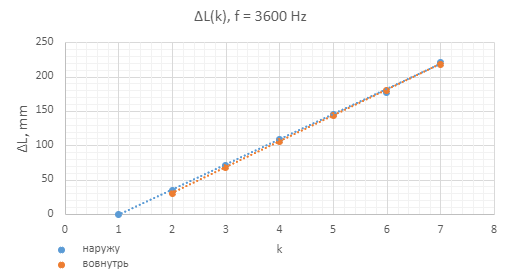
\includegraphics[width=10 cm]{coplot2.PNG}
    \label{fig:coplot2}
\end{figure}
\begin{figure}[h]
    \centering
    \begin{center}
    \end{center}
    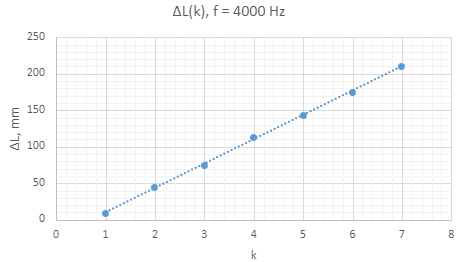
\includegraphics[width=10 cm]{coplot3.PNG}
    \label{fig:coplot3}
\end{figure}
\begin{figure}[h]
    \centering
    \begin{center}
    \end{center}
    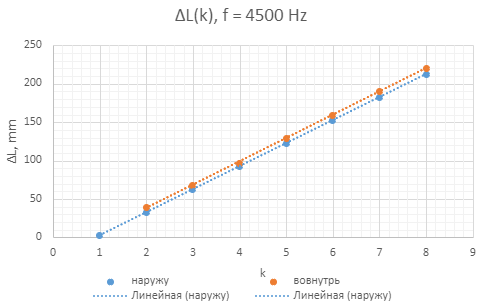
\includegraphics[width=10 cm]{coplot4.PNG}
    \label{fig:coplot4}
\end{figure}
\begin{figure}[h]
    \centering
    \begin{center}
    \end{center}
    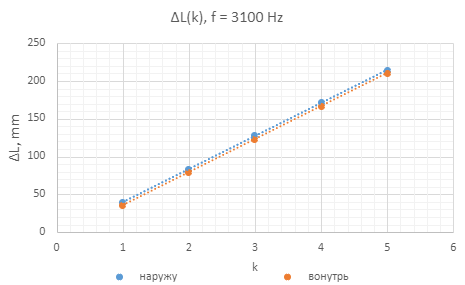
\includegraphics[width=10 cm]{coplot5.PNG}
    \label{fig:coplot5}
\end{figure}
\newpage

Вычислим с помощью полученных графиков скорость звука в углекислом газе и рассчитаем погрешности. Погрешность $\sigma_{c}$ отдельного измерения определяется следующей формулой:
$$ \sigma_{c} =c \sqrt{\Big(\frac{\sigma_{L}}{L}\Big)^2+ \Big(\frac{\sigma_{A}}{A}\Big)^2},$$
где $A$ - коэффициент наклона прямой на графике.

$$c = (270\pm3)\frac{\text{м}}{\text{с}}.$$

\textbf{Измерения с включенным термостатом}
\begin{figure}[h]
    \centering
    \begin{center}
    \end{center}
    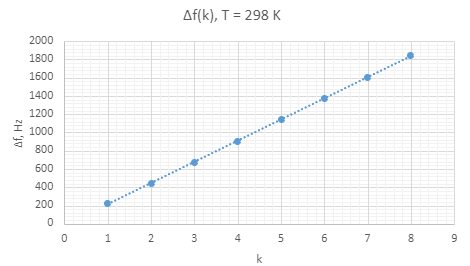
\includegraphics[width=10 cm]{tplot1.PNG}
    \label{fig:tplot1}
\end{figure}
\begin{figure}[h]
    \centering
    \begin{center}
    \end{center}
    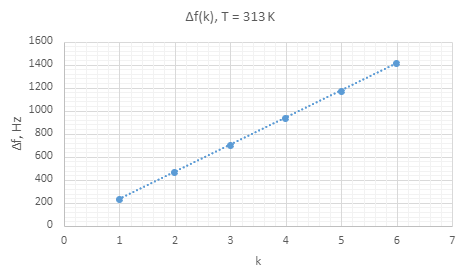
\includegraphics[width=10 cm]{tplot2.PNG}
    \label{fig:tplot2}
\end{figure}
\begin{figure}[h]
    \centering
    \begin{center}
    \end{center}
    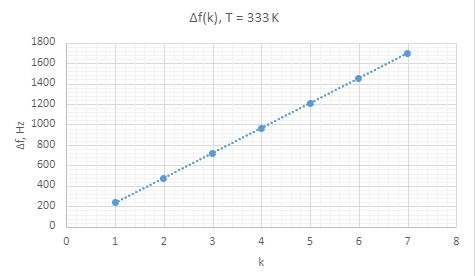
\includegraphics[width=10 cm]{tplot3.PNG}
    \label{fig:tplot3}
\end{figure}
\begin{figure}[h]
    \centering
    \begin{center}
    \end{center}
    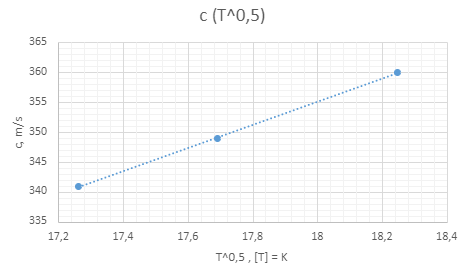
\includegraphics[width=10 cm]{ctplot340.PNG}
    \label{fig:ctplot340}
\end{figure}
\newpage

По полученным данным расчитаем $\gamma$.
$$\overline{\gamma} = 1.423$$
$$\gamma_{сл} = \sqrt{\frac{\sum_{i=1}^{4} (\gamma_{i}-\overline{\gamma})^2}{3}} = 0.04 .$$
Косвенная погрешность определения $\gamma$ мала, так как $\frac{2\sigma_c}{4c} \approx 0.25 \%.$
Итак, $$\gamma = 1.42 \pm 0.04 ,$$ что в пределах погрешности совпадает  с теоретическим значением $\gamma = 1.4 .$
Если обратить внимание на полученные значения для $c$, то можно усомниться в справедливости формулы $c^2 = \frac{\gamma R T}{\mu}$ и начать предпологать, что показатель адиабаты является функцией от температуры $\gamma = \gamma(T)$. Однако температуры в данном опыте не слишком большие и другие степени свободы не могли активироваться у молекул газа. Есть гипотеза, объясняющая такие разбросы.Вероятно измерения производились не во время достижения термодинамического равновесия и нужно было ждать приличное время (~5 минут) после того как на термостате установится необходимая температура, для того чтобы система пришла в пригодное состояние для измерений.

\section{Вывод}
Мы научились измерять показатель адиабаты через скорость звука с помощью резонансных пиков зависимости амплитуды принимаемого сигнала при прохождении в закрытом пространстве от расстояния, проходимого звуком в одну сторону из-за появления стоячих волн, результаты эксперимента совпали с табличными значениями. 
\end{document}

